%%%%%%%%%%%%%%%%%% USAGE INSTRUCTIONS %%%%%%%%%%%%%%%%%%
% - Compile using LuaLaTeX and biber, unless there is a particular reason not to. Do not use the older LaTex/PDFLaTeX or BibTeX. (The fonts won't work correctly.)
% - Font and the report 'year' must be specified when all \documentclass or the template won't work correctly. (There's no error checking/default cases!)
% - For best performance save images/graphics as PDF files, not as png/jpg/eps. This makes no difference to how images are inserted using \includegraphics.
% - As many further packages as wanted can be loaded. Below are just an example set. Note that template itself loads a number of packages, including hyperref.
% - References are handed using biblatex.
% - Link to the presentation of theses policy: https://documents.manchester.ac.uk/DocuInfo.aspx?DocID=2863

%%%%%%%%%%%%%%%%%% META DATA SETUP %%%%%%%%%%%%%%%%%%
% This is where the document title and author are set. Other details for the title page are set later
% Note that if/when you edit these you may need to 'Recompile from scratch' to get the changes to display in the PDF. (In Overleaf, select the down arrow to the right of the 'Recompile' button)
\begin{filecontents*}{\jobname.xmpdata}
    \Title{Development of Two Wheel Self Balancing Platform for Monocular Vision Based Trajectory Tracking} % title of your thesis
    \Author{Winston Scott 107067151} % should be student number rather than name to help with annoymous marking
    \Language{en-GB}
    \Copyrighted{True}
    % More meta-data fielda can be added here if wanted, see https://ctan.org/pkg/pdfx?lang=en for fields
  \end{filecontents*}
  %%%%%%%%%%%%%%%%%% DOCUMENT SETUP %%%%%%%%%%%%%%%%%%
  \documentclass{uom_eee_dissertation_casson} 
  %%%%%%%%%%%%%%%%%% PACKAGES AND COMMANDS %%%%%%%%%%%%%%%%%%
  % Packages
  \usepackage{graphicx,psfrag,color} % for postscript graphics files
    \graphicspath{ {./DesingImgs/} }
  \usepackage{amsmath}               % assumes amsmath package installed
    \allowdisplaybreaks[1]           % allow eqnarrays to break across pages
  \usepackage{amssymb}               % assumes amsmath package installed 
  \usepackage{url}                   % format hyperlinks correctly
  \usepackage{rotating}              % allow portrait figures and tables
  \usepackage{multirow}              % allows merging of rows in tables
  \usepackage{lscape}                % allows pages to be typeset in landscape mode
  \usepackage{tabularx}              % allows fixed width tables
  \usepackage{verbatim}              % enhanced version of built-in verbatim environment
  \usepackage{footnote}              % allows more control over footnote environments
  \usepackage{float}                 % allows H option on floats to force here placement
  \usepackage{booktabs}              % improve table line spacing
  \usepackage{lipsum}                % for adding dummy text here
  \usepackage[base]{babel}           % for proper hypthenation in lipsum sections
  \usepackage{subcaption}            % for multiple sub-figures in a single float
  % Add your packages here
  %\usepackage{pdfcomment}            % for alt text for accessibility
  \usepackage{booktabs}              % for better looking tables
  % Then to add images use:
  % \pdftooltip{\includegraphics[width=0.5\textwidth]{image.pdf}}{Alt-text here}
  % This makes the text in the image non-select-able though (assuming it's a vector file)
  
  % Custom commands
  \newcommand{\degree}{\ensuremath{^\circ}}
  \newcommand{\sus}[1]{$^{\mbox{\scriptsize #1}}$} % superscript in text (e.g. 1st)
  \newcommand{\sub}[1]{$_{\mbox{\scriptsize #1}}$} % subscript in text
  \newcommand{\sect}[1]{Section~\ref{#1}}
  \newcommand{\fig}[1]{Fig.~\ref{#1}}
  \newcommand{\tab}[1]{Table~\ref{#1}}
  \newcommand{\equ}[1]{(\ref{#1})}
  \newcommand{\appx}[1]{Appendix~\ref{#1}}
  %%%%%%%%%%%%%%%%%% REFERENCES SETUP %%%%%%%%%%%%%%%%%%
  % Setup your references here. Change the reference style here if wanted
  \usepackage[style=ieee,backend=biber,backref=true,hyperref=auto]{biblatex}
  % Note backref=true adds a page number (and hyperlink) to each reference so you can easily go back from the references to the main document. You may prefer backref=false if you need to stick strictly to a given reference style
  % Fixes which can't be applied in the .cls file
  \DefineBibliographyStrings{english}{backrefpage = {cited on p\adddot},  backrefpages = {cited on pp\adddot}}
  %  \renewcommand*{\bibfont}{\large}
  % Add more .bib files here if wanted
  \addbibresource{References.bib}
  
  %%%%%%%%%%%%%%%%%% START DOCUMENT %%%%%%%%%%%%%%%%%%
  % Don't edit these lines, title and author are automatically taken from the document meta-data defined above
  \begin{document}
  \makeatletter
  \title{\xmp@Title}
  \studentid{\xmp@Author}
  \makeatother
  
  % Set the below yourself
  \course{Mechatronics and Robotics Engineering}  % "Master of Science in" is added automatically
                                                     % Our courses are: Advanced Control and Systems Engineering, Advanced Control and Systems Engineering with Extended Research, Communications and Signal Processing, Communications and Signal Processing with Extended Research, Electrical Power Systems Engineering, Advanced Electrical Power Systems Engineering, Renewable Energy and Clean Technology, Renewable Energy and Clean Technology with Extended Research
  \submitdate{2025}                                  % regulations ask only for the year, not month
  \wordcount{1000}		                            % use \wordcount{} to set the count, \thewordcount to print in the text
  \maketitle

  %%%%%%%%%%%%%%%%%% LISTS OF CONTENT %%%%%%%%%%%%%%%%%%
  \uomtoc
  % other lists are not required, but can include \uomlof and \uomlot if really want to

  %%%%%%%%%%%%%%%%%% ABSTRACT %%%%%%%%%%%%%%%%%%
  \begin{abstract} % put abstract here. Limit is 1 page.
    The highly dynamic Two Wheel Self Balancing Robot (TWSB)
    has a large exploration space for high level control strategies. 
    This reports presents an autonomous line racing TWSB utilizing 
    a monocular vision system on low cost hardware. 
    Cascaded PID and LQR controllers 
    are explored as a SISO and MIMO control strategies. 
    Discussion on software architecure 
    for rapid develoepemtn on  emmbeded platoforms is also presented. 
    An efficient line tracking algorithm is developed based 
    on the SNR of a curvilinear transformation of the image, 
    and is compared with common classical computer vision approaches.
    The system is tested in a variety of conditions 
    and demonstrates robustness to disturbances 
    and can suitably track a line at high speeds.
    \begin{figure}[H]
    \includegraphics[height=\textwidth]{bBot ISO Drawing v3.pdf}
    \caption{3D CAD Render of the TWSB system}
    \end{figure}

  \end{abstract}%
  \clearpage
  %%%%%%%%%%%%%%%%%% SECTION 1 %%%%%%%%%%%%%%%%%%
  \section{Introduction}
    The TWSB system is an example of a non-linear, under-actuated system which is inherently unstable[1].
    Compared to a differential drive platform, the TWSB's dynamics are more complex, enabling a 
    wider range of high level robotic behaviors to be explored. \cite{RoboLimbo} []. 
    The extra degree of freedom 
    presents some challenges when vision based control strategies are used. 
    Techniques from [] and [] from the field of quad-rotor attitude control are explored to minimize the effect 
    of the fundamental instability of the system.

    This paper presents the design developemtn and validionof a TWSB robotic platform for automonus line racing. 
    The system is designed to be low cost and easily aseembeld whilst providing suitabel protection, as testing 
    of racing lines may lead to large forces on the system, fig(1)

    
    As such many control strategies have been proposed to stabilize the system.[] 
    Of these the most common are the LQR and Cascaded PID controllers. 
    


    Amongst the early works on the TWSB system,[1] achieved telle-operation on flat ground. 
    This was implemented using a FPGA base DSP system. Advances in price to performance of emmbeded systems and MEMS sensors have allowed 
    [][][] to similarly obtain remote control of the TWSB system using a low powered microcontroller.
    Having a stable platform and available computational resources, higher levels of autonomy can be developed. 
    []Utilizes a camera as a matrix of binary intensity sensors and a rule based algorithm to successful track 
    a line whilst balancing. [] Developed an end to end neural network to perform the same task and [] proposes 
    a ConvNet based approach which utilizes all of the cameras RDB-D data to be able to 
    autonomously navigate with human-centric social behavior. 
    To the same end, [][][] develop wheeled robot navigation and realtime lane segmentation geometric computer vision techniques. 
    [][] build a online data driven model of the mobile system and embed it in a ModelPredictive controller. This adaptive control strategy 
    is shown to be robust to un-modeled environment and plant dynamics, allowing for autonomous aggressive maneuvers. 
    This is implemented on a commercial GPU which allows for realtime operation of the optimization algorithm.
    \pagebreak{}




  %%%%%%%%%%%%%%%%%% SECTION 2 %%%%%%%%%%%%%%%%%%
  \section{Literature review} % edit section heading as appropriate

    \subsection{Introduction}

    This is now a MIMO control problem. numerous control strategies have been used to solve this problem, 
    with different goals in mind. [dadsasd] presents a lqr controller which tracks 
    the desired velocity, lending itself to tele-operative use cases, [sadasda] 
    shows how a cascaded PID controller is used to perform position control, 
    and [aasdasd] explores how a neural net can be used for swing up and balance control.
    \subsection{Summary}
  %%%%%%%%%%%%%%%%%% SECTION 3 %%%%%%%%%%%%%%%%%%
  \pagebreak{}
  \section{Mathematical Modeling} % edit section heading as appropriate
    Significant research, both in simulation[][] and 
    application[][][] has been done on the 1DOF inverted pendulum
    on a cart as a bench mark for control techniques[]. This is often used as a baseline model for the TWSB problem
    however higher order models are required to capture the dynamics of the TWSB system. [] Explores models of different fidelity 
    and [] expands on this and developed a 3DOF model by decoupling the system based into 2 controllers which 
    operate on the yaw and pitch rate independently. [trajectory tracking control for navigation of the inverse pendulum type] 
    \pagebreak{}
    \subsection{DC Motor Model}    
    \begin{figure}[H]
        \centering
            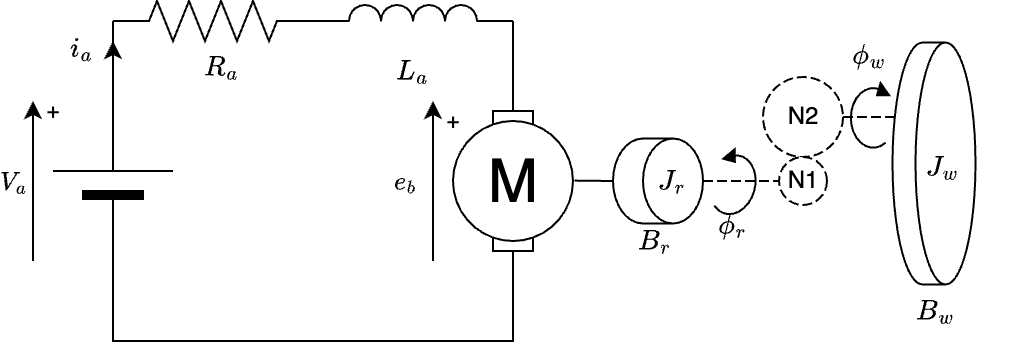
\includegraphics[width=0.75\textwidth]{DCMotorModel.png}
        \caption{Gearbox DC Motor Model Diagram}
    \end{figure}
    The system is driven by two independently voltage controlled DC motors through planetary gearboxes, 
    as is shown in Fig(2). 
    DC motors execute a torque $t_r$, proportional to the armature current $i_a$, when a voltage $V_a$ is applied.
    The ratio of motors inductance $L_a$ and resistance $R_a$ determine the time constant $\tau_e$ of the motor. 
    That is the time it takes for $i_a$ to reach 63.2\% of its final value. []
    The gear box has a gear ratio $N_1/N_2$ which amplifies the viscous damping coefficient $B_G$ and the moment of inertia $J_G$  with respect to the motor.

    The speed of the gearbox, $\dot\phi_w$ is related to the armature voltage by the well-known transfer function  Kt/(s*((Jm*s+Bm)*(La*s+Ra)+(Kt*Ke)))
    \begin{equation}
        \begin{aligned}
            \frac{\Omega_w \left(s\right)}{V_a \left(s\right)}=\frac{K_t }{s^2 \cdot L_a R_a +\;s\left(R_a \cdot J_{\mathrm{eq}} +B_{\mathrm{eq}} \cdot L_a \right)+K_t {\cdot K}_e +R_a \cdot B_q }\cdot n
        \end{aligned}
    \end{equation}
    Where $\Omega_w$ is the laplace transform of the output speed, $J_r$ is the moment of inertia of ththe rotor.
    The rotors viscous damping $B_r$ is assumed to be negligible, as is $B_G$. 
    For small motors, $t\tau_e$ is small hence $L_a << R_a$ and the motor can be approximated as a first order system as in 
    \begin{equation}
        \begin{aligned}
            \frac{\Omega_w \left(s\right)}{V_a \left(s\right)}=\frac{K_t }{s\cdot R_a + \left(J_G +{J_r \cdot \left(N_1/N_2\right)}^2 \right)+K_t K_e }\cdot\left(N_1/N_2\right)
        \end{aligned}
    \end{equation}

    \pagebreak{}


    \subsection{2DOF System Model}

    \begin{figure}[H]
        \includegraphics[width=\textwidth]{ModelingDiags.pdf}
        \caption{2DOF Model}
    \end{figure}

    The TWSB robot is modeled as two separate 2DOF systems as shown in fig(4), 
    namely a wheeled inverted pendulum (WIP) and a differential drive robot (DDMR).
    It however exits in a 3D space, and for the purposes of this paper must be able to rotate about the inertial Z axis. 
    [] Shows that that is possible to separate the steering control from the balance control 
    without linear velocity and direction angular velocity being constrained too much. 
    [] conducts a 2DOF model of the WIP which  decouples the effect of yaw rate from the pitch rate. 

    The system equations of motion in the WIP case are developed through the Lagrangian Method [][][] are shown to be 
    
    The system of equations () are linearized around the equilibrium point $\theta\approx 0$  and after standard algebraic manipulation the 
    2DOF state space representation of the system is given by eq(6).


   
    \pagebreak{}

    \subsection{System Design}
        \begin{figure}[H]
            \includegraphics[width=\textwidth]{bBot Drawing v3.pdf}
            \caption{CAD Drawing of the TWSB system}
        \end{figure}

        The TWSB body is 3D printed out of PLA plastic in 3 parts for minimal assembly.
        The battery pack is quickly swappable and both it and the electronics sub assembly 
        are soft-mounted in a roll cage like housing for protection against impacts. 
        \begin{figure}[H]
            \includegraphics[width=\textwidth]{SystemOverview.pdf}
            \caption{System Overview}
        \end{figure}

        Two brushed DC motors are powered by an H bridge IC 
        The STM32F411RE Microcontroller Unit (MCU) is used to control the 
        motors and monitor the 6 Axis IMU over I2C. It communicates with the 
        Raspberry Pi 5 over UART via a custom ASCII protocol discussed in section 3.3. 
        The system is powered by a a nominal 12V Li ion Battery pack. A USB-C CC-CV charger is used for quick 
        and accessible recharging,critical for mobile robotics applications. Battery Voltage is monitors by the MCU
        and the pack is protected by a BMS and a 3A poly-fuse.
        A simple circuit adapted from[] is used to safely load share between the battery pack and the charger.


        \pagebreak{}
        \subsubsection{System Identification}


        A series of experiments are conducted in order to obtain an estimate transfer function of the motors
        
        \begin{table}
                \begin{tabular}{|r|c|c|c|c|c|c|}
                    \vline 
                    Gear Ratio & Rated Torque & Rated Speed & Rated Current & Stall Torque & Stall Current \\
                     1:20 & 0.39 & 400 & 500 & 2 & 0.15 \\
                    \vline
                \end{tabular}
                \caption{DC Motor Parameters}
        \end{table}


        \begin{figure}[H]
            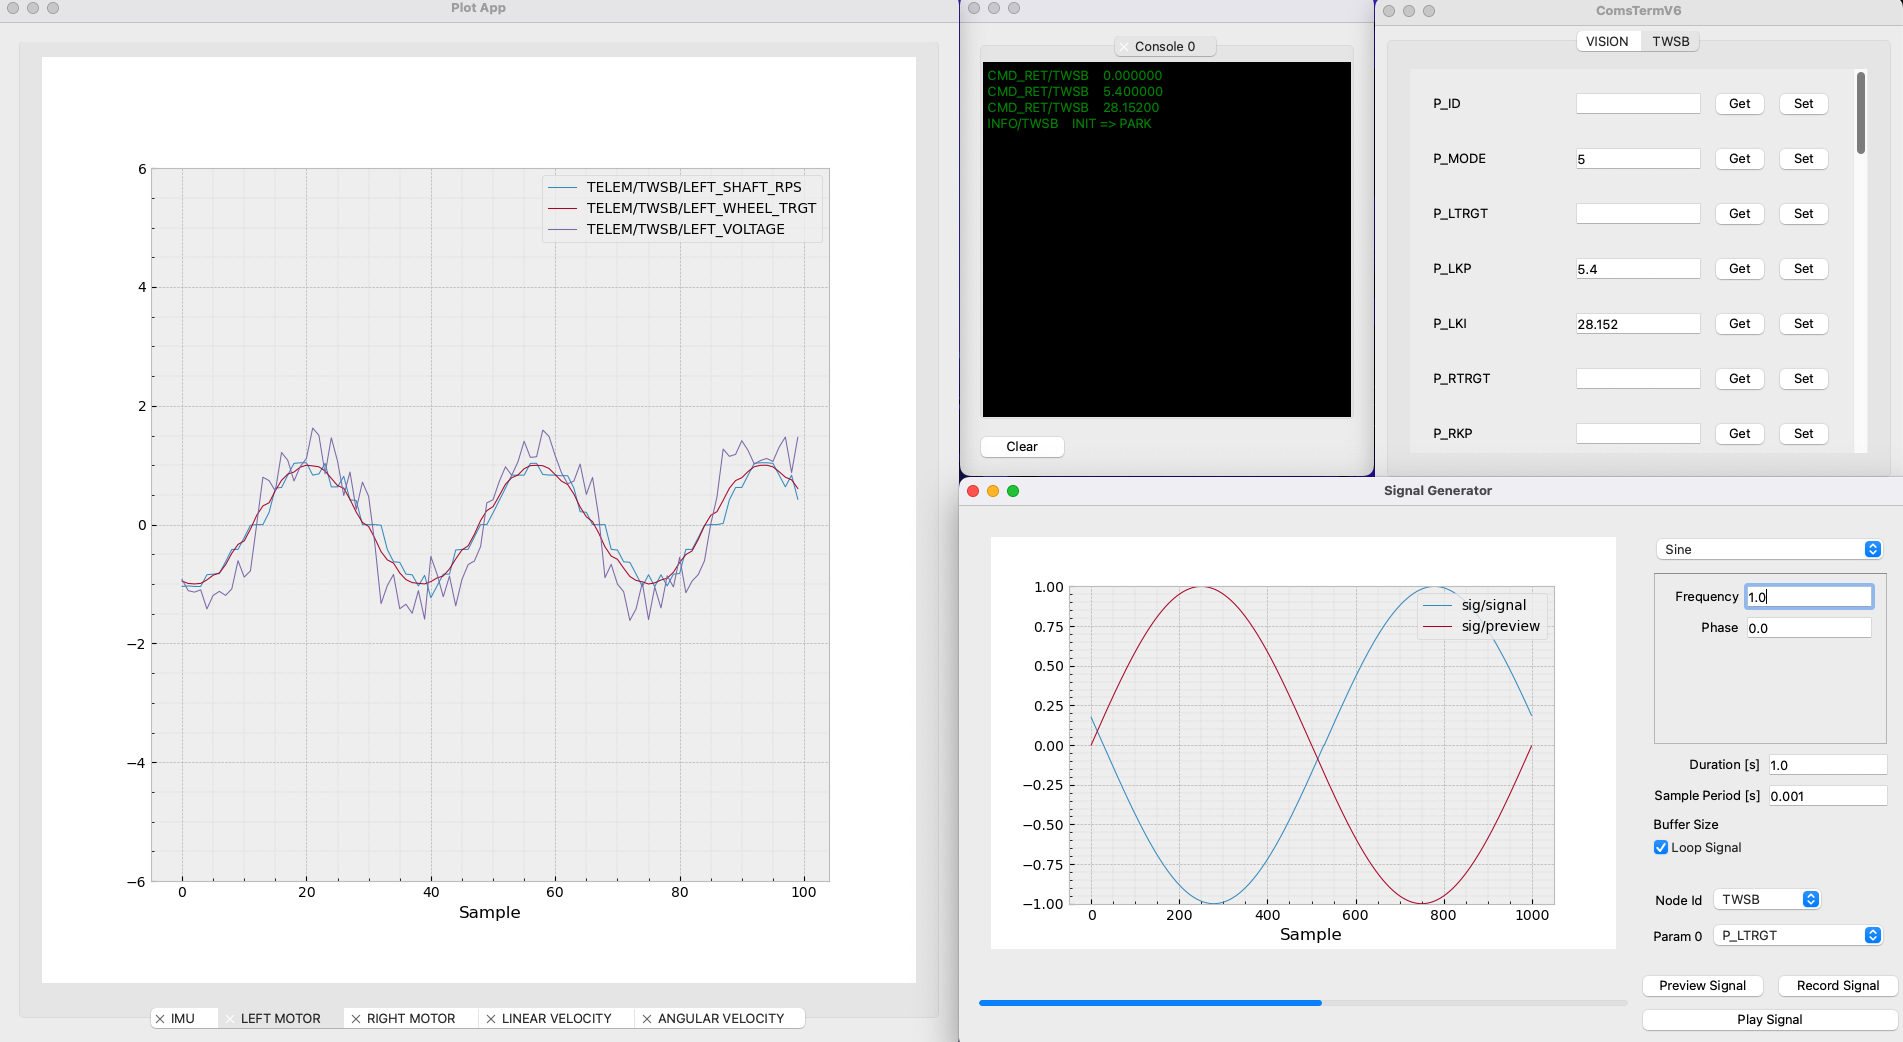
\includegraphics[width=\textwidth]{SysIDMotorSetUp.png}
            \caption{System Identification Setup}
        \end{figure}
        Using the test bench setup shown in fig(6), a series of reference ramp, step, 
        sine and chirp inputs are applied to each of the DC motors. 

        \begin{figure}[H]
            \centering
            \subfloat{
                \includegraphics[width=0.3\textwidth]{openstep.pdf}
            }
                \subfloat{
                \includegraphics[height=0.2\textwidth]{speed_voltage_DCMotor.pdf}
            }
            \subfloat{
                \includegraphics[width=0.3\textwidth]{openChirp.pdf}
            }
            \caption{Open Loop Speed Voltage experiments}
        \end{figure}    
        The resulting data, shown in fig(7) is then used by the linear system identification toolbox in MATLAB 
        to obtain the transfer function of the DC motors as 
        \begin{equation}
            \begin{aligned}
                \frac{\Omega_w \left(s\right)}{V_a \left(s\right)}=\frac{K_t }{s\cdot R_a + \left(J_G +{J_r \cdot \left(N_1/N_2\right)}^2 \right)+K_t K_e }\cdot\left(N_1/N_2\right)
            \end{aligned}
        \end{equation}



        \pagebreak{}
        \subsubsection{Parameters }
        The system parameters are given in table(1). 
        The masses of the sub-compoentes obtanined by weighing,
        and estimates of the 3D printed parts mass are given by the slicer software. 
        The CAD Model computes the center of mass using these values and the COM is identified in fig(6).
        The using the approximate model as in fig(2) the moment of inertial is computed from standard formulas.
        \begin{table} [H]
            \centering
            \begin{tabular}{|c|c|c|c|}
                \hline
                Parameter & Value & Units & Description \\
                \hline
                $m$ & 1.5 & kg & Mass of the body \\
                $l$ & 0.1 & m & Length of the body \\
                $J_b$ & 0.01 & $kgm^2$ & Moment of inertia of the body \\
                $r$ & 0.03 & m & Radius of the wheel \\
                $d$ & 0.132 & m & Wheel base \\
                $R_a$ & 1.5 & $\Omega$ & Resistance of the motor \\
                $K_t$ & 0.01 & Nm/A & Torque constant of the motor \\
                $K_v$ & 0.01 & V/rad/s & Back EMF constant of the motor \\
                $J_w$ & 0.01 & $kgm^2$ & Moment of inertia of the wheel \\
                \hline
            \end{tabular}
            \caption{System Parameters}
        \end{table}

       
        
        \pagebreak{}
        \subsection{Software Architecture}
        The modern standard for robotics software is the Robot Operating System 2 (ROS2)[]. 
        Whilst this is a powerful tool, it is deemed too complex for the requirements of this project.
        Nevertheless some core concepts are used such as its 
        decentralized message pattern shown in fig(7). ZeroMQ[] is used for 
        anonymous pub sub style communication between computational nodes.
        \begin{figure} [H]
            \includegraphics[width=\textwidth]{CommunicationDataPath.pdf}  
            \caption{InterProcess Communications Data Path}
        \end{figure}

        The software is managed by systemd through services. 
        Several self-diagnosis tools are used for resource monitoring and auto recovery. 
        For example both the MCU and the CPU monitor each other using watchdog timers.
        Programs implement a runtime Remote Procedure Call (RPC) ASCII interface using 
        a GET/SET/RUN pattern operating on runtime parameters. This significantly reduces the compile/flash/debug 
        iteration time. A Gstreamer pipeline is setup a RSTP server which can be accessed on the network.
        Core functionality is implemented in C++17. 
        \begin{figure} [H]
            \includegraphics[width=\textwidth]{FirmwareArch.pdf}
            \caption{Firmware Architecture}
        \end{figure}
        Key components of the firmware are shown in fig(8).
        It is implemented in c99 using the libopencm3 project[]. 
        The MCU also presents the same RPC ASCII interface over serial.
        The super-loop executes commands at 20Hz, 
        and publishes its state at 100Hz.

        The data-aquististion system obtains a timestamped sample of the TWSB state 
        and telemetry values sampled by the MCU through the serial link.
        This results in non-uniformly sampled data. Parsing the UART IO buffer on Linux 
        and timestamp is bottlnekced by the CPU. An event driven system is used to minimize CPU overhead.   
        Worst case jitter is observed, under CPU stress tests[] to be 1ms. This is acceptable for telemetry data, but
        any further online or offline signal processing is resampled to a uniform rate using lagrange interpolation \cite{DataStreamProcessing.}
        \pagebreak{}
    \subsection{State Estimation}
        Given the model in eq(6) and the system parameters in table(1) the 2DOF 
        state space representation of the system is given by eq(7).
        \subsubsection{Sensors Overview}
        The TWSB system uses an Kalman Filter to obtain an estimate of theta, 
        from the accelerometer and gyroscope readings of the IMU. 
        This is polled at the maximum 1kHz using an interrupt according to the IMU datasheet[]. 
        The kalman estimate is obtanined by eq(8)  after initilay observingin
         a prediction and then an inovation step.
        The state ransiion model is givenby [] as eq(9).  The system is initialized with a 
        priori estimates of the state and covariance matrix. in eq(10-11). 

        Fig(9) shows that the ertiamte stabalizses after 1 second, 
        and is robust to noise from the acceleroemter. 
        \pagebreak{}
    \subsection{Control System}
       
        A simple PID controller opperatign on the pitch error is often enough to stabilize one of the systems dynamic variables[].
        However as shown by fig3, x position drifts. Since the linear velocity is coupled to the
        pitch angle by eq(1), the pitch angle must be controlled to maintain a constant x velocity. 

        \subsubsection{Cascade PID}

        The TWSB achieves balance by osculating the pitch angle about the vertical axis. 
        The lineariezed system of equatiosn in eq(4) is applicable 
        only when the pitch angle is small, this is taken to be 10 degrees. 
        A target maximum pitch oscitation is set to +-1 degree. 
        The TWSB also needs to be able to move along the $X'$ axis in its inertial frame.
        This is achieved by regulating the pitch angle about equilibrium or 0 degrees.

        A cascaded pid controller is used to control the pitch angle and the linear velocity. 
        If the inner loop dynamics are much faster than the outer loop, 
        then the inner loop can be approximated as a disturbance[].



        In order to determine the maximum operating frequency of the outer loop, 
        the inner motor speed loop is closed at 200Hz and the system is observed.
        
        Through the Ziegler-Nichols method[], the PID gains for each DC Motors speed control loop 
        are obtained as shown in table(2). This process however may cause damage to the motors 
        during the sustained oscillations at the critical gain. 
       
        

        

        The frequency response of the transfer function is shown in fig(4) and its closed loop bandwidth is determined to be rads

        This is then used to obtain the PID gains in table(4) in MATLAB using pole-placement techniques
        \begin{table}[H]
            \centering
            \begin{tabular}{|c|c|c|}
                \hline
                Parameter & Zeigler-Nichols & SysId \\
                \hline 
                $K_p$ & 0.1 & 0.1 \\
                $K_i$ & 0.01 & 0.01 \\
                $K_d$ & 0.01 & 0.01 \\
                \hline
            \end{tabular}
            \caption{PID Gains}
        \end{table}

        A P controller is used to regulate the steering control signal, which modeled
        as a disturbance from the 2D dynamics model.

        The error of the pitch angle is regulated by a PID controller operating at 100Hz. 
        
        This results in a stable system in 1DOF space, controlling the body velocity requires the outermost loop to be closed at 20Hz.
        The final cascaded closed loop pid controller is shown in fig(5) with the gains in table(5)

        \begin{figure}[H]
            \includegraphics[width=\textwidth]{CascadedPID.pdf}
            \caption{Cascaded PID Controller}
        \end{figure}

        \begin{table}[H]
            \centering
            \begin{tabular}{|r|r|r|r|c|c|c}
                \hline
                & \multicolumn{4}{c|}{Process Variable}  \\
                \hline
                Parameter & $v_b$ & $\theta$  & $\omega_L$ & $\omega_R$ \\
                \hline      
                $K_p$ & 0.1 & 0.1 & 0.1 & Nm \\
                $K_i$ & 0.01 & 0.01 & 0.01 & Nms \\
                $K_d$ & 0.01 & 0.01 & 0.01 & Nm/s \\
                \hline
            \end{tabular}
            \caption{PID Gains}
        \end{table}
        \pagebreak{}
        \subsubsection{LQR}
        A Linear Quadratic Regulator (LQR) is used to control the system in 2DOF space.
        The system is linearized around the operating point given in eq(5) 
        and the state space representation is given by eq(6).
        Selecting the Q and R matrixes as eq(7) and eq(8) respectively, 
        the K feedback matrix in eq(9) is obtained by solving the Algebraic Riccati
        equation of the discretized system eq(10) in MATLAB.

         

    \subsection{Vision System}
        \subsubsection{Curvilinear Transformation}
        The planar two wheel self balancing robot, now modeled as a point P, subject to the differential drive constraints, 
        can be instantaneously described as following some segment or radius r. This arc segment forms part of a continuous spline. 
        The curvature of the spline is given by the inverse of the radius of the circle that best fits the arc segment.
        Where a positive curvature indicates a right turn and a negative curvature indicates a left turn.
        The forward direction is x, and left if y. using the side of the angle between the robots heading and the observed center line can be used as the derivative term.
        adding the curvature K, 
            \subsubsection{Camera Calibration}
            \begin{figure}
            \includegraphics[width=\textwidth]{PinHoleModel.pdf}
            \caption{Pin Hole Camera Model}
            \end{figure}

            \subsubsection{IMU Based Software Stabilization Methods}
            \subsubsection{Perspective Transformation}
            \begin{figure}
            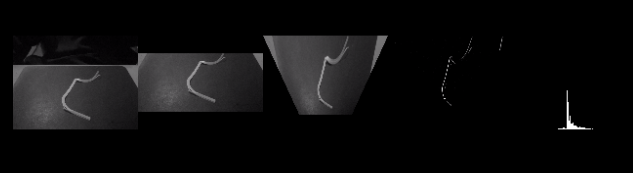
\includegraphics[width=\textwidth]{VisionPipelineRes.png}
            \end{figure}
            \subsubsection{Polynomial Fitting}
            \subsubsection{Trajectory Generation}

    \subsection{Trajectory Tracking}
        \subsubsection{Pure Persuit}
        \begin{figure}
            \includegraphics[width=\textwidth]{PurePersuit.pdf}
            \caption{Pure Pursuit Algorithm}
        \end{figure}
        \subsubsection{Model Predictive Control}


  %%%%%%%%%%%%%%%%%% SECTION 4 %%%%%%%%%%%%%%%%%%
  \section{Results and discussion} % edit section heading as appropriate
    \subsection{Introduction}
    \subsection{Balance Performance}
    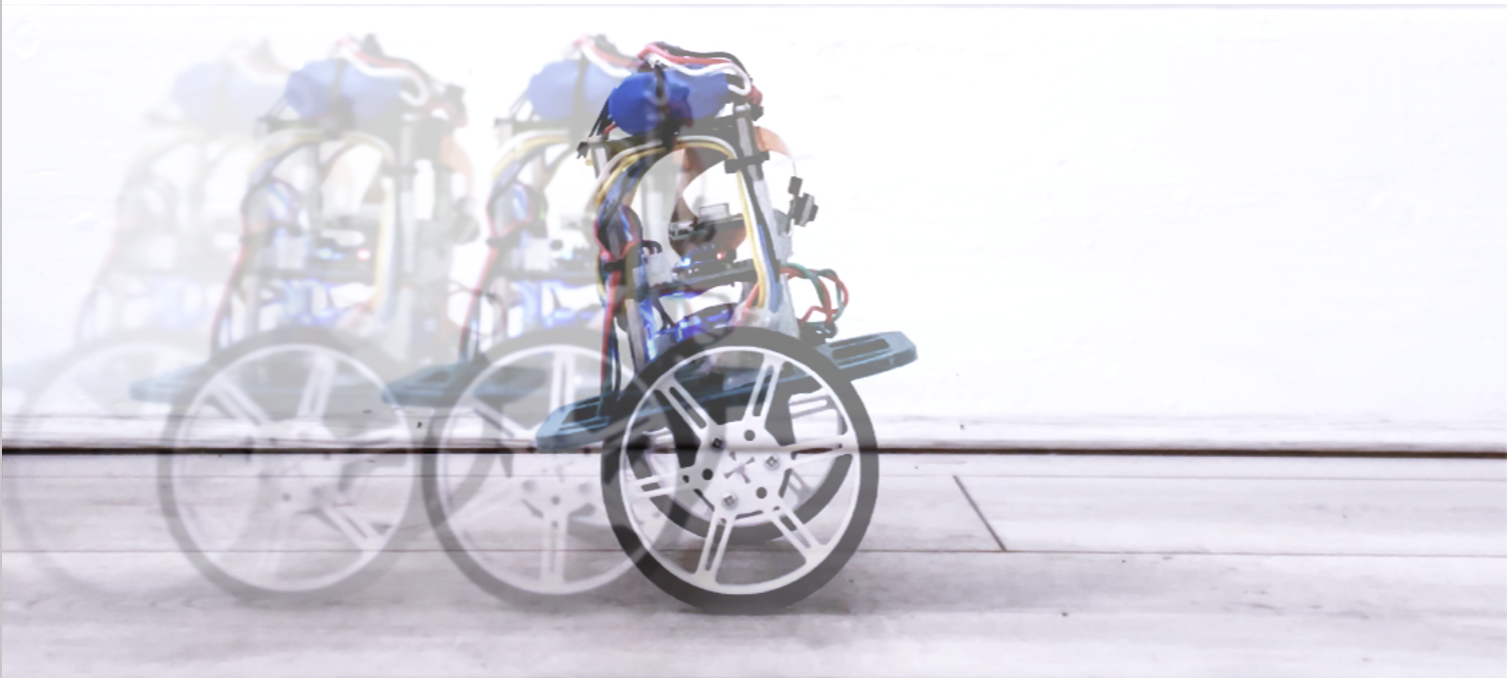
\includegraphics[width=\textwidth]{V1Colated.png}
    \subsection{Operational Robustness}
    \subsection{Line Trajectory Tracking}
    \subsection{More detail}
    \subsection{Summary}
  %%%%%%%%%%%%%%%%%% SECTION 5 %%%%%%%%%%%%%%%%%%
  \section{Conclusions and future work} % edit section heading as appropriate
    \subsection{Conclusions}
      \subsection{Future work}
  %%%%%%%%%%%%%%%%%% REFERENCES %%%%%%%%%%%%%%%%%%
  clearpage % uncomment to start on a new page if wanted
  \printbibliography[title={References},heading=bibintoc] % a single list of references for the whole thesis
  %%%%%%%%%%%%%%%%%% APPENDICES %%%%%%%%%%%%%%%%%%
  \begin{uomappendix} 
      \section{Code}
      \section{Risk assessment}
      Risk assessment is a required appendix. Put here.
      %\section{Other appendices as necessary}
  \end{uomappendix}
  
  %%%%%%%%%%%%%%%%%% END MATTER %%%%%%%%%%%%%%%%%%
  \end{document}